\section{各詳細}
\subsection*{松島}
\addcontentsline{toc}{subsection}{松島}
\footnotesize

\textbf{松島}は,仙台市から車で約30分ほどの距離に位置する美しい観光地で,特にその景観と歴史的な価値で知られている.
松島は日本三景の一つに数えられ,数百の小島が点在する風光明媚な海岸線が特徴である.

\begin{figure}[H]
	\centering
	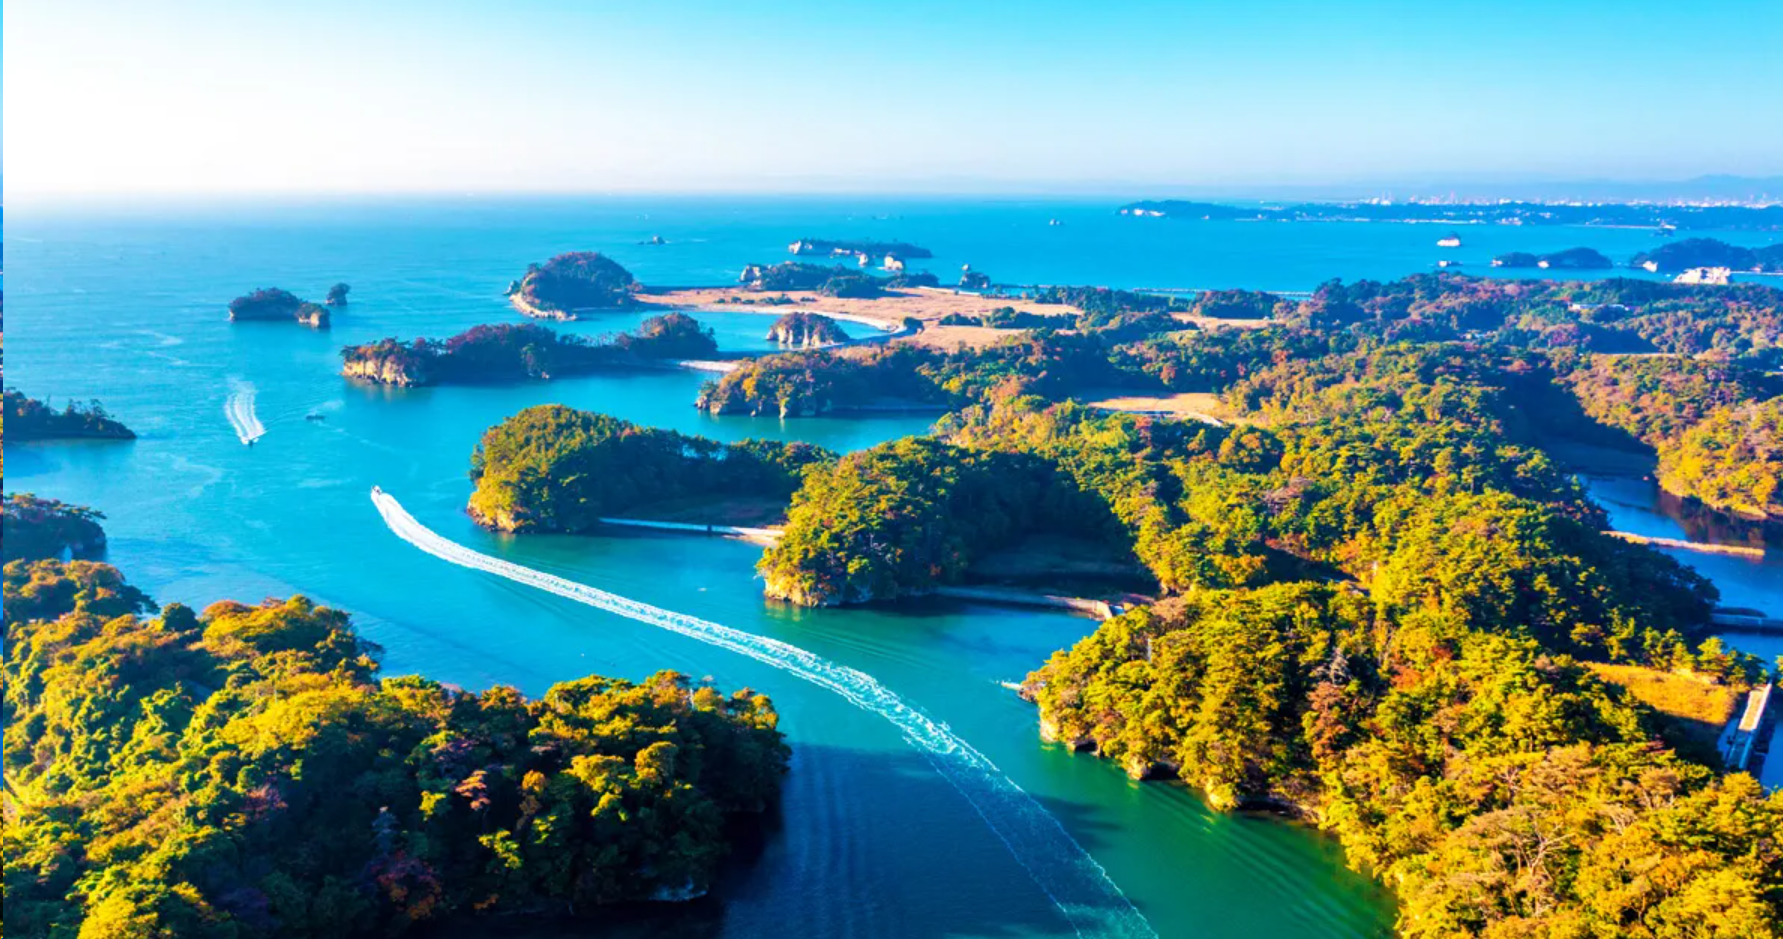
\includegraphics[width=0.7\linewidth]{img/matsushima-islets}
	\label{fig:matsushima-islets}
\end{figure}

松島の最大の魅力は,その景観である.
松島湾には約260の小島があり,四季折々の風景が楽しめる.
特に秋の紅葉や冬の雪景色は別格であり,多くの観光客が訪れる.
松島の景観は,松の木々と海の青さが織りなすコントラストが美しく,訪れる人々を魅了する.

\begin{figure}[H]
	\centering
	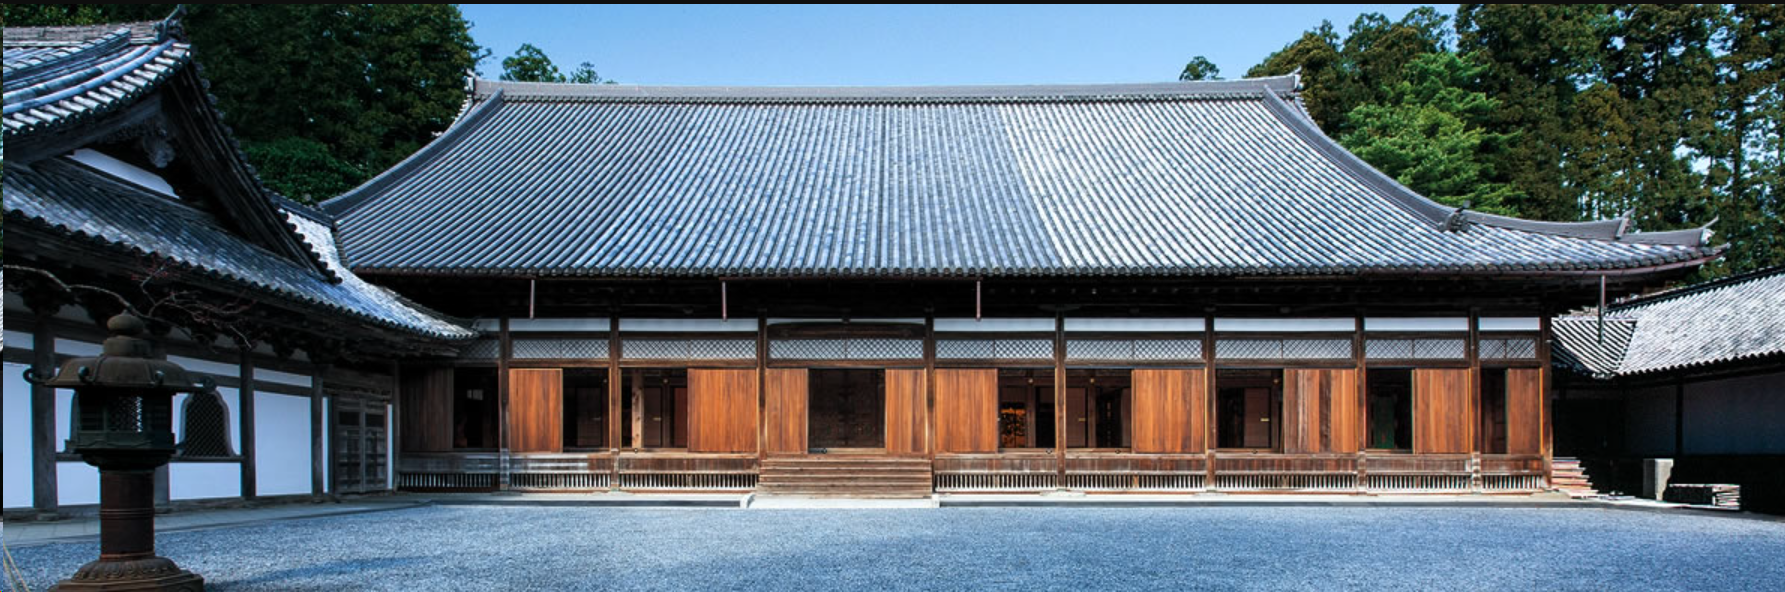
\includegraphics[width=0.8\linewidth]{img/zuiganji}
	\label{fig:zuiganji}
\end{figure}

松島には多くの歴史的名所がある.
とくに有名なものに,松島のシンボルともいえる\textbf{五大堂}がある.
この堂は松島の景観を一望できる場所に位置し,観光客に人気のスポットである.
また,松島には\textbf{\ruby{瑞巌寺}{ずいがんじ}}という重要文化財もあり,歴史的な建物や庭園が見どころだ.
\newpage

\subsection*{大崎八幡宮}
\addcontentsline{toc}{subsection}{大崎八幡宮}

\textbf{大宮八幡宮}は平安時代の初期に創建されたとされ,長い歴史を持つ神社である.
神社の主祭神は\ruby{八幡神}{やはたのかみ}であり,武運や商売繁盛を祈願するために多くの人が訪れる.
また,神社の建物は江戸時代に再建されたもので,豪華な装飾や彫刻が施されている.
特に,重要文化財に指定されている本殿は見事な技術で作られており,訪れる人々を魅了する.

大崎八幡宮では,年間を通じてさまざまな祭りや行事が行なわれる.
とくに有名なのは,毎年行なわれる\textbf{大崎八幡宮例大祭}で,地元の人々や観光客が集まり,\ruby{神輿}{しんよ}\footnote{神社で行なわれるお祭りの際に神霊を載せて担ぐ乗り物.\ruby{御輿}{みこし}とも呼ばれる.} や伝統的な踊りが披露される.
また,初詣や七五三,結婚式など,個人の祈願や祝い事にも利用され,多くの人々に親しまれている.
\begin{figure}[H]
	\centering
	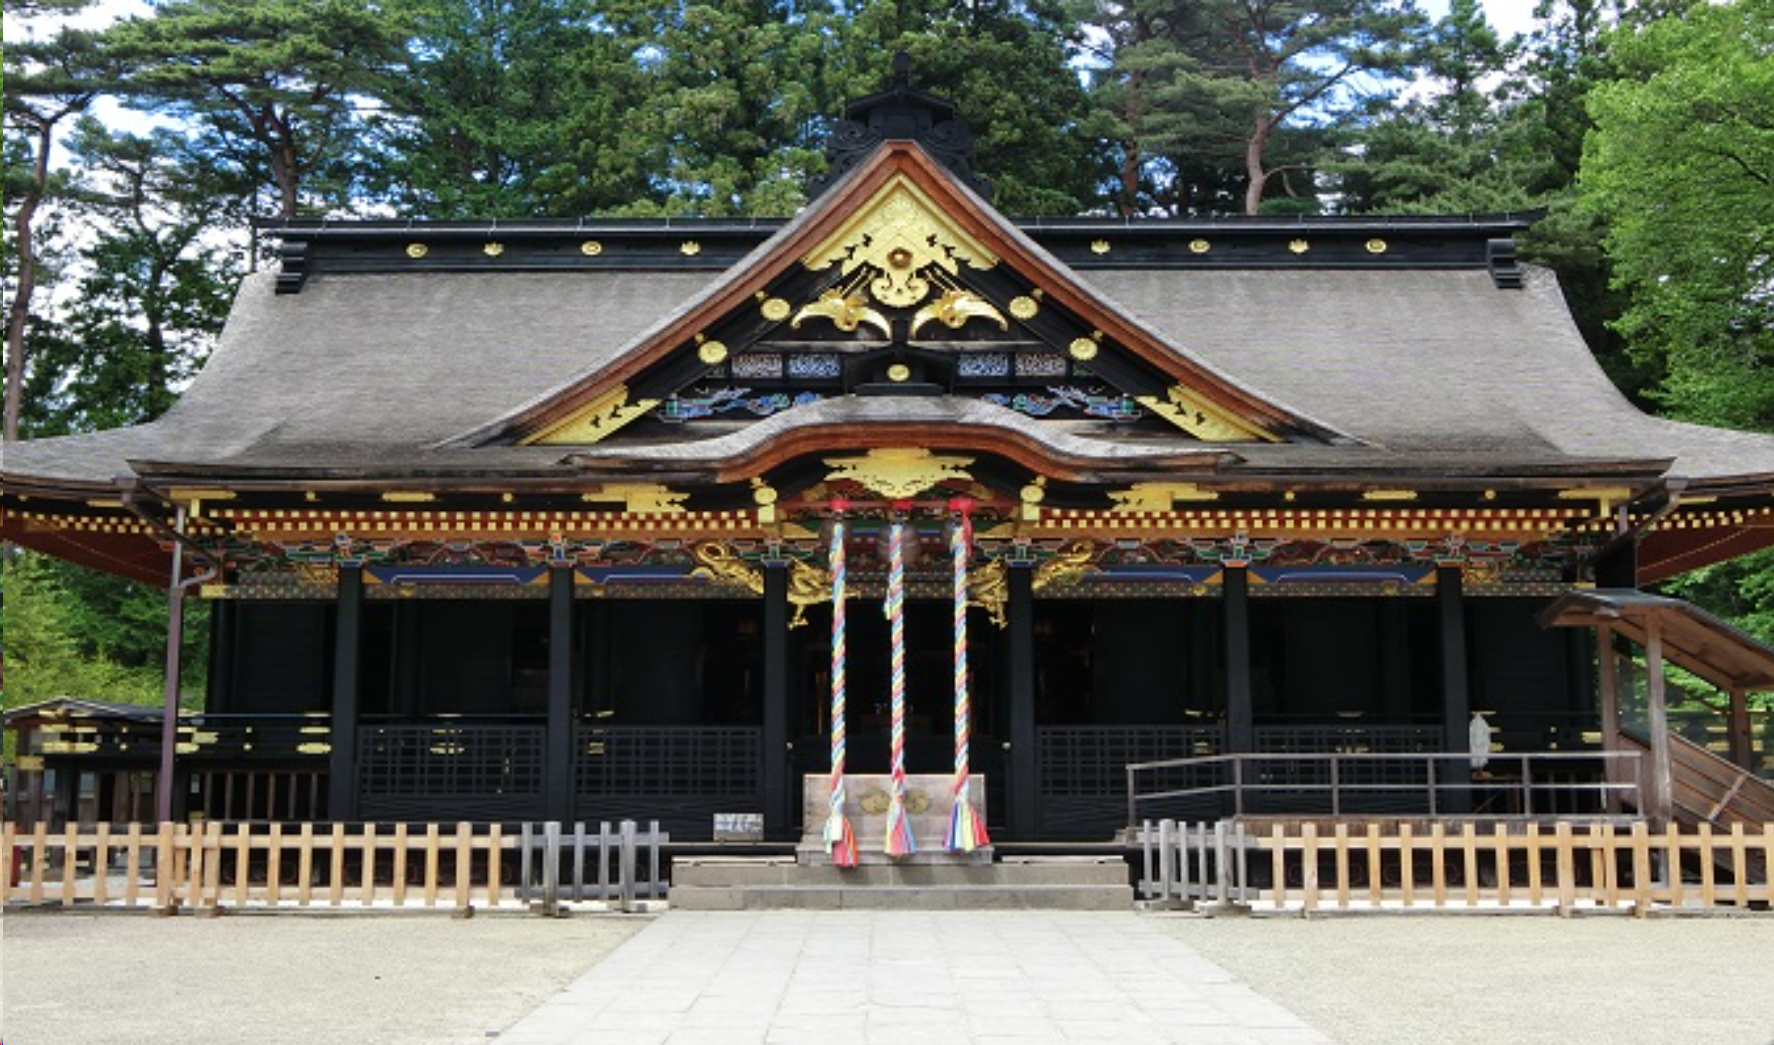
\includegraphics[width=0.8\linewidth]{img/osakimachimangu}
	\label{fig:osakimachimangu}
\end{figure}

大崎八幡宮は,歴史的な価値と自然の美しさを兼ね備えた場所であり,訪れる人々にとって特別な体験を提供している.
神社の静かな雰囲気の中,心を落ち着け,祈りをささげることができる貴重なスポットである.
ぜひ一度訪れて,その魅力を体感してみるとよい.
\newpage

\subsection*{伊達政宗}
\addcontentsline{toc}{subsection}{伊達政宗}

\begin{figure}[H]
	\centering
	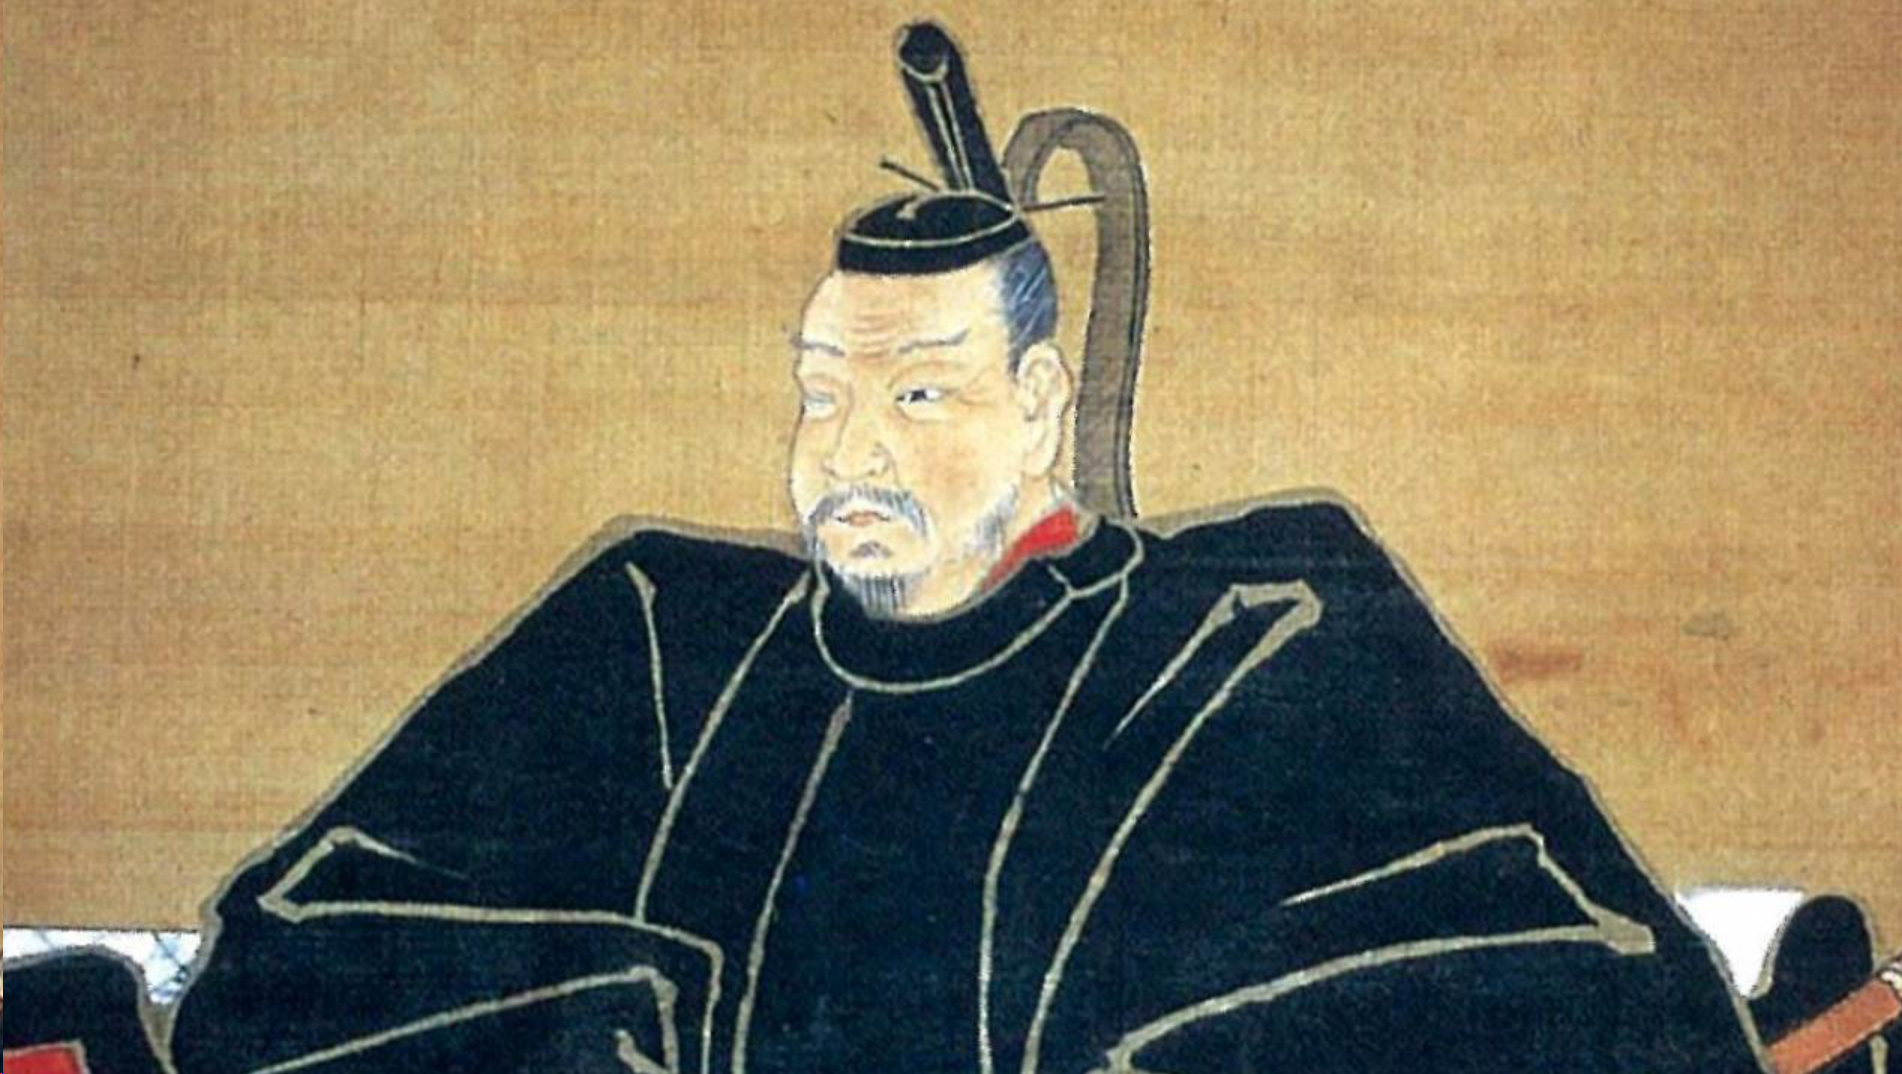
\includegraphics[width=0.7\linewidth]{img/datemasamune}
	\label{fig:datemasamune}
\end{figure}


\textbf{伊達政宗}は戦国時代の日本の著名な武将であり,特に東北地方の支配者として知られる.
1521年に生まれ1590年に亡くなるまでの間に,独自の政治的手腕と軍事的才能を発揮した.
政宗は,特にその戦略的な思考と外交能力で知られ,彼の治世下で仙台藩を築き上げた.

政宗は,幼少期に片目を失ったことから,\textbf{独眼竜}と呼ばれるようになった.
彼は,父である伊達\ruby{輝宗}{てるむね}の後を継ぎ,家族の名声を高めるために多くの戦闘に参加した.
政宗は周囲の大名との同盟を結び,また敵対する勢力に対しても果敢に戦った.
特に,彼は豊臣秀吉の下での戦いに参加し,その後の関ケ原の戦いにも影響を与えた.

\begin{figure}[H]
	\centering
	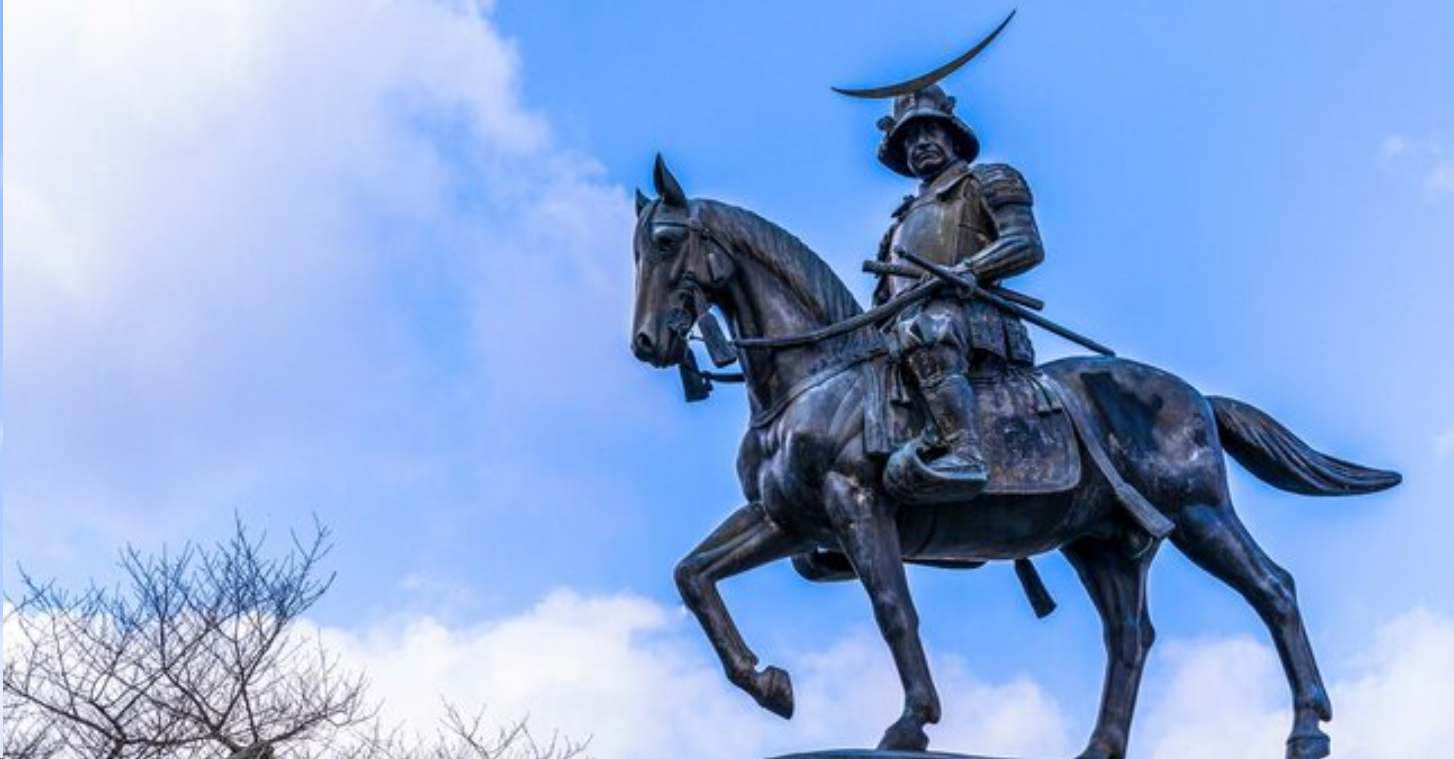
\includegraphics[width=0.6\linewidth]{img/datemasamunezou}
	\label{fig:datemasamunezou}
\end{figure}

政宗の政治的な手腕は,彼の領地である仙台を発展させることに寄与した.
彼は商業や文化の発展を促進し,仙台を東北地方の中心地として位置づけた.
また,彼はキリスト教の布教にも関心を持ち,宣教師を受け入れるなど,国際的な視野を持った人物でもあった.
\newpage

\subsection*{食文化}
\addcontentsline{toc}{subsection}{食文化}

仙台の\textbf{ずんだ}と\textbf{牛タン}は,地域の食文化において非常に重要な役割を果たしている.
これらの料理は,仙台の歴史や文化と深く結びついており,観光客にも人気がある.

\begin{figure}[H]
	\centering
	\begin{minipage}[b]{0.49\columnwidth}
		\centering
		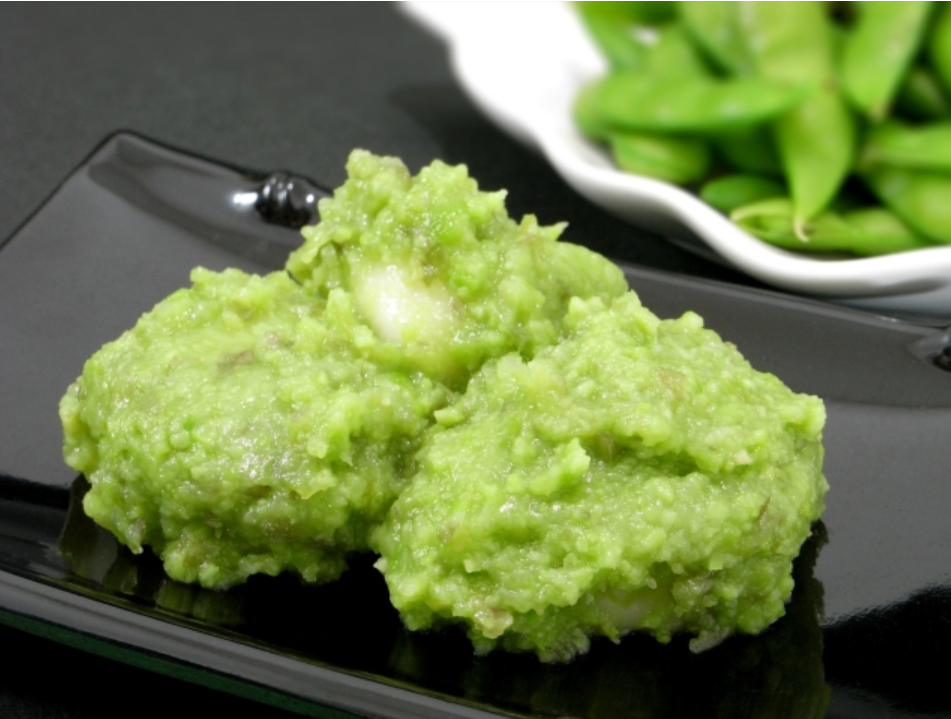
\includegraphics[width=0.9\columnwidth]{img/zundamochi.png}
		\label{fig:zundamochi}
	\end{minipage}
	\begin{minipage}[b]{0.49\columnwidth}
		\centering
		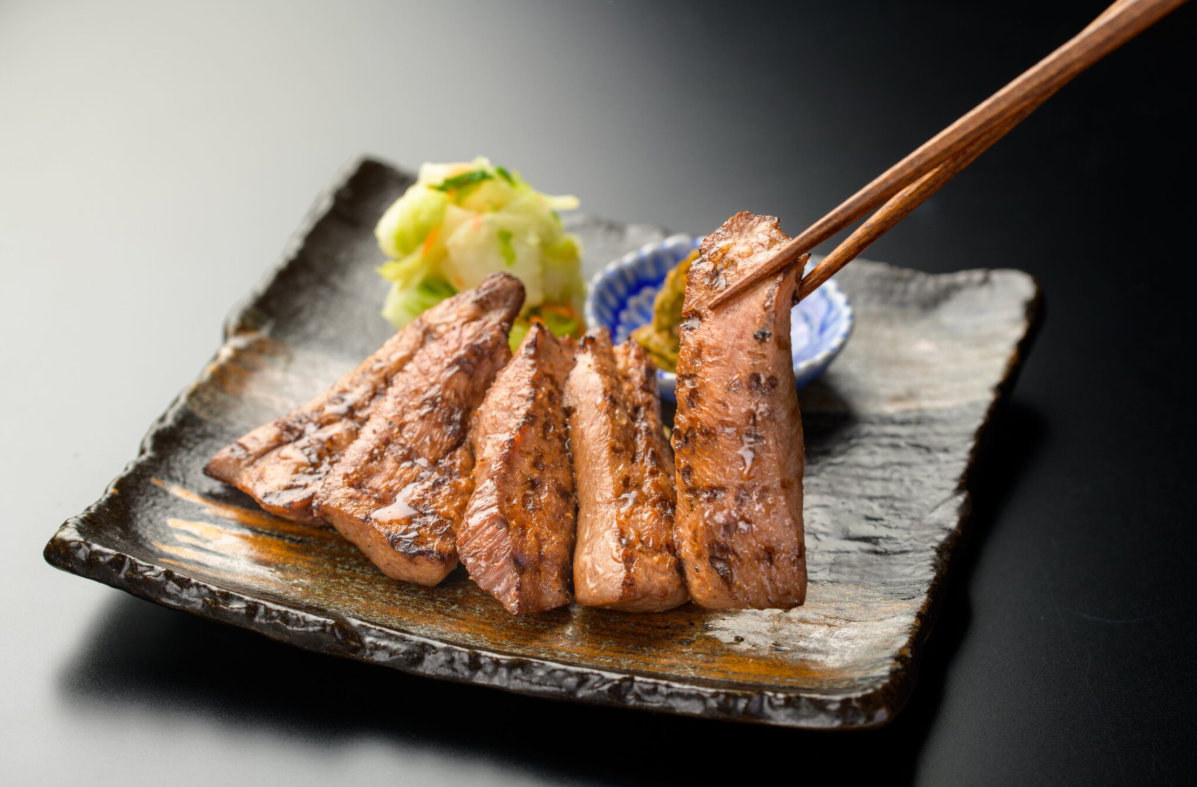
\includegraphics[width=0.9\columnwidth]{img/gyutan-yaki.png}
		\label{fig:gyutan-yaki}
	\end{minipage}
\end{figure}

\subsubsection*{ずんだの歴史}
ずんだは,主に枝豆を使ってペーストで,甘さと独特の風味が特徴である.
ずんだの起源は江戸時代に遡るとされ,当初は農作業の合間に食べられていたと考えられる.
特に,仙台藩の藩士たちが好んで食べていたことから,仙台の名物として広まった.
ずんだの名の由来は,「豆を打つ」の「豆打(づだ)」や,伊達政宗が\ruby{陣太刀}{じんだち}の柄で豆を潰したとの伝説から来た「陣太(じんだ)」が訛って「ずんだ」になったなど,さまざまな説がある.

\subsubsection*{牛タンの歴史}
戦後の1950年代(太平洋戦争が集結し,日本が復興に向けて歩み始めた昭和23年),アメリカの駐在軍が多かった仙台には,大量の牛肉が運び込まれていた.
その中,名店「太助」の初代店主 故・佐野啓四郎氏が洋食で使われていた牛タンの旨さに虜になり,試行錯誤の上,今なお定番となっている\textbf{牛タン焼き}が誕生した.
仙台のローカル定食として誕生した牛タン焼きは,高度経済成長の時代,転勤や出張で仙台にやってきたサラリーマンたちの評判が次第に広がり,マスメディアに取り上げられ,「仙台名物」として全国に広まったとされている.
\newpage
